\documentclass[parskip=full]{scrartcl}

\usepackage{pdfpages}
\usepackage[utf8]{inputenc}
\usepackage[T1]{fontenc}
\usepackage[german]{babel}
\usepackage{hyperref}
\hypersetup{
	pdftitle={Pflichtenheft},
	bookmarks=true,
}
\usepackage{csquotes}

\usepackage{fancyhdr}%<-------------to control headers and footers
\usepackage[a4paper,margin=1in,footskip=.25in]{geometry}
\fancyhf{}
\fancyfoot[C]{\thepage} %<----to get page number below text
\pagestyle{fancy} %<-------the page style itself

\usepackage{xcolor}
\usepackage{framed}
\definecolor{shadecolor}{RGB}{220,220,220}
\usepackage{float}


\title{Android GO! App - Pflichtenheft}
\author{Gruppe 3}
\date{11.06.17}

% define custom lists
\usepackage{enumitem}
\usepackage{lipsum}

\makeindex

\begin{document}

\begin{titlepage}
	\begin{center}
	{\scshape\LARGE \bfseries Entwurfsdokument \par}
	\vspace{1cm}
	{\scshape\Large Praktikum der Softwareentwicklung \\ Sommersemester 2017\par}
	\vspace{1.5cm}
	{\huge\bfseries Android GO! App\par}
	\vspace{2cm}
	{\Large\itshape - Gruppe 3 -\par}
	\vfill
	{\bfseries erstellt von:\par}
	Arsenii Dunaev \\
	Florian Kröger \\
	Tina Maria Strößner \\
	Volodymyr Shpylka \\	
	\vfill
	% Bottom of the page
	{\large 09.07.17 \par}	
	\end{center}
\end{titlepage}

\newpage

\begin{abstract}
Die Android App GO! ist eine mobile Applikation, die speziell zur Organisation von Treffen (z. B. gemeinsames Essen im Café oder in der Mensa) entwickelt wird. Beim erfolgreichen gemeinsamen Losgehen wird der gemittelte GPS-Standort von Mitgliedern der Gruppe angezeigt.\\

Dieses Dokument erläutert den Entwurf des Systems auf der Grundlage des Pflichtenhefts.
\end{abstract}

\newpage

\tableofcontents

\newpage

\section{Änderungen zum Pflichtenheft}

Es wurden im Entwurf folgende Änderungen gegenüber dem Pflichtenheft vorgenommen:
\begin{enumerate}
	\item \textbf{Produktdaten - Benutzer} \\
	Es werden in den Produktdaten zusätzlich eine (von Firebase automatisch generierte) InstanceID gespeichert, die es dem Server erlaubt, Daten an das Android-Gerät eines bestimmten Benutzers zu senden.
	\item \textbf{Detailansicht der GOs} \\
	Es ist jedem Mitglied einer Gruppen (unabhängig von Teilnahmestatus) möglich, die Detailansicht eines GOs aufzurufen. Um den Karten-Tab öffnen zu können, um die Standorte der anderen Teilnahmer zu verfolgen, gilt weiterhin, dass der Teilnahmestatus 'Bestätigt' oder 'Unterwegs' lauten muss.
\end{enumerate}

\newpage

\section{Architekturstil und Paketstruktur}

\subsection{Client}
Die Architektur der Client-Applikation orientiert sich am Model-View-ViewModel (MVVM) Muster. Dies wird auf Android-Systemen durch die, auch hier eingesetzten, Architecture Components unterstützt. Das untenstehende Paketdiagramm zeigt den groben Aufbau der Client-Applikation, welche Abhängigkeiten bestehen und welche Aufgaben jedes Paket übernimmt. Genauere erläuterungen hierzu finden sich in den darauffolgenden Abschnitten.

\begin{figure}[H]
	\centering
	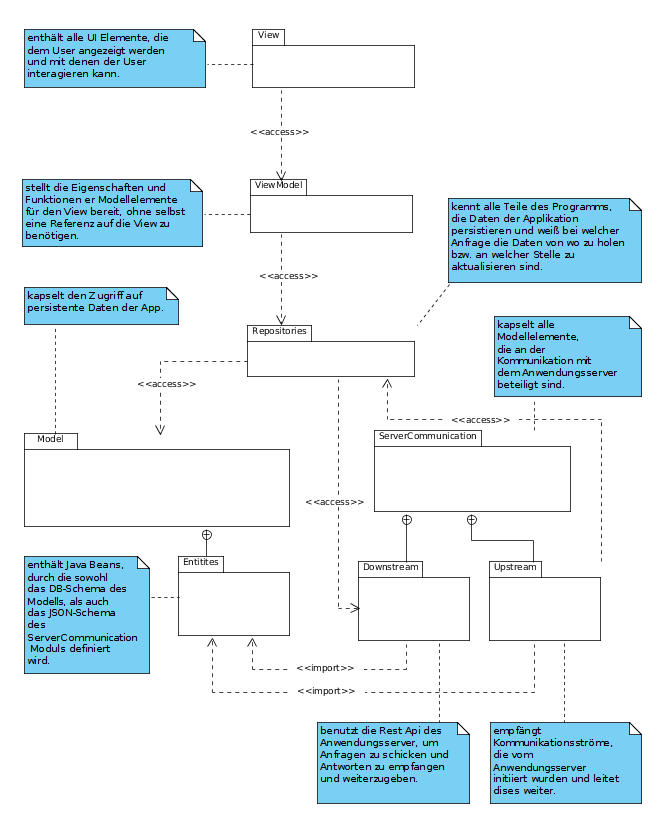
\includegraphics[scale=0.5]{../Klassendiagramme/paketdiagramm_client.png}
	\caption{Paketdiagramm der Clientanwendung}
\end{figure}

\subsubsection{Views}
Das Paket Views enthält alle Klassen, die am User Interface des Benutzers beteiligt sind. Das sind sämtliche Activities, Fragments und dazugehörige .xml-Layouts. Das Modul ist für die Präsentation der Appdaten sowie die Implementierung der Präsentationslogik (Umsetzung der Eigenschaften der Daten und Weiterleitung von Benutzereingaben) zuständig.

\textbf{Abhängigkeiten zu anderen Paketen:}\\
Das Paket Views kann die Informationen, die dem Benutzer angezeigt werden, nicht selbst generieren, sondern bekommt diese bereitgestellt von den entsprechenden ViewModells.

\textbf{Unterpakete:}\\
das Paket enthält das Unterpaket 'RecyclerView'. Da in der Applikation viele (verschiedene) RecyclerViews verwendet werden, gibt es für die Erstellung derselben ein eigenes Paket, dessen Aufgabe es ist, von den Datenobjekten die das Model liefert die gewünschten Informationen zu extrahieren und diese mit dem richtigen Layout zusammenzuführen. Innerhalb des Pakets besteht eine Abhängigkeit derjenigen View-Klassen, die einen RecyclerView verwenden zu dem Unterpaket RecyclerViews. Das Unterpaket RecyclerViews selbst ist nocht von anderen Klassen und Paketen abhängig.

\subsubsection{Modell}
Das Modell ist die Datenzugriffsschicht der Applikation, d.h. sie kapselt den Zugriff auf persistente Daten, die in einer lokalen SQLite Datenbank gehalten werden.Darüber hinaus enthält das Paket die Geschäftslogik der App, das hei?t hier werden die om ViewModel aufbereiteten und weitergeleiteten Befehle umgesetzt und anschließend die sich ergebenden Datenänderungen an das ViewModell zurückgegeben. Die Modellklassen, die sich lokal in der Applikation befinden, werden erweitert durch das Datenmodell, welches sich auf dem Server befindet. Es muss stets die Datenkonsistenz dieser zwei Modellteile sichergestellt werden (vgl. Paket Repository).

\textbf{Abhängigkeiten zu anderen Paketen}\\
Der Aufbau und die Operationen, die auf der lokalen Datenbank durchgeführt werden, werden mittels des Frameworks \textit{Room} realisiert.

\textbf{Unterpakete:}\\
Das Modell enthält das Unterpaket 'Entities'. Dies enthält die Java Entitäten, die von Room zu den Relationen der Datenbank umgesetzt werden. Die Datenbank kann von Room auch ohne eine Implementierung der Zugriffslogik aufgebaut werden. Die Entities haben demnach keine Anhängigkeiten zu anderen Klassen innerhalb des Programms. DIe Zugriffslogik der DAOs setzt hingegen die Existenz der Datenbank voraus, es gibt eine Abhängigkeit vom Modell zu den Entities.

\subsubsection{ViewModell}
Das ViewModell ist das Bindeglied zwischen View und Modell. Es tauscht Informationen mit dem Modell aus und stellt so der View öffentliche Eigenschaften und Befehle zur Verfügung, die an die Steuerungselemente der UI angebunden werden können. Dabei hat as ViewModell keine Referenz auf die View. Durch diese lose Kopplung kann die View jederzeit ausgetauscht werden, ohne dass das ViewModell verändert werden muss.

\textbf{Abhängigkeiten zu anderen Paketen}\\
Das ViewModell benötigt eine Referenz zum Modell, um die von der View empfangenen Befehle weiterleiten und die richtigen Daten von Modell anfordern zu können. Um diese Abhängigkeit zu entkoppeln und das Ansprechen der richtigen Modellkomponente zu erleichtern, wird diese Abhängigkeit über einen Vermittler ("Repository") geleitet. Dies ermöglicht das einfache Austauschen des Modells, ohne dass das ViewModell verändert werden muss.

\subsubsection{ServerCommunication}
Das Paket ServerCommunication übernimmt die Kommunikation der App mit dem Server, also das Speichern von Daten auf dem Server bzw. das Holen von Daten von dem Server. Darüber hinaus werden in diesem Paket auch Nachrichten, die vom Server gesendet werden empfangen und an das Modell zur Verarbeitung weitergeleitet.

\textbf{Abhängigkeiten zu anderen Paketen}\\
Das Paket hat keine Abhängigkeiten zu anderen Paketen der Applikation. Die Implementierung des REST-Clients erfolgt über das Framework \textit{Retrofit 2}. Hier besteht also eine Abhängigkeit zu einem externen Framework. Außerdem benötigt das Modukl zur fehlerfreien Ausführung seiner Aufgaben ein funktionierendes Backend (REST-Api, das die entsprechenden Ressourcen bereitstellt) des Systems.

\textbf{Unterpakete:}\\
Das Modul ServerCommunication setzt sich aus zwei Untermodulen zusammen. Das Modul \textit{Upstream} implementiert die Kommunikation, die über die REST-Api des Tomcat-Servers läuft, also jegliche Kommunikation, die von einem Client initiiert wird. Das Modul \textit{Downstream} hingegen ist dafür zuständig Kommunikationsströme zu empfangen, die vom Server initiiert werden und diese den Vermittlern zur Verbreitung weiterzuleiten.

\subsubsection{Repositories}
Wie in den vorherigen Abschnitten erläutert, ist die Geschäftslogik der App aufgeteilt auf den lokalen Teil (Modell) und einen Remote-Teil (ServerCommunication), die miteinander synchronisiert werden müssen. Zusätzlich müssen die ViewModells nach sämtlichen Änderungen mit den aktuellsten Daten versorgt werden. Dise Abhängigkeiten der einzelnen Komponenten werden in den Repository-Klassen zusammengefasst. Genauere Erläuterungen zur Funktionsweise finden sich in Abschnitt \ref{Vermittler}.

\textbf{Abhängigkeiten zu anderen Paketen:}\\
...

\subsection{Server}
Die Architektur ser Servers orientiert sich an einer MVC-Architektur. Das Programm des Servers ist in folgende Pakete aufgeteilt:
\begin{itemize}
	\item CommunicationLayer
	\item BusinessLayer
	\item PersistenceLayer
\end{itemize}

\subsubsection{CommunicationLayer}
Dieses Paket übernimmt die Rolle des Views. Die CommunicationLayer vereint alle Klassen, die an der Kommunication mit den Clients beteiligt sind. Es besteht aus den Unterpaketn Upstream und Downstream. Die Klassen des Pakets Upstream sind dafür zuständig, ein REST-API zur Verfügung zu stellen und auf Anfragen der Clients zu antworten, d.h. die Kommunikation wird von den Clients initiiert. Das Downstream-Paket hingegen schickt Nachrichten an Clients, ohne vorher von diesen angesprochen worden zu sein. Hierf"ur wird der Firebase Cloud Messaging Service benutzt.

\subsubsection{BusinessLayer}
Die BusinessLayer ist der Controller der Serveranwendung. dieses Modul realisiert Datenänderungen und Operationen auf der PersistenceLayer. Außerdem ist hier die Logik für die Erfassung und Auswertung der Standortdaten implementiert. Dies funktioniert ohne die Beteiligung des Modells, da diese Daten nur kurzfristig erfasst, verarbeitet und zurückgesendet werden müssen.

\subsubsection{PersistenceLayer}
Die PersistenceLayer bildet das Datenmodell. Sie ist für die Speicherung der Daten zuständig, sowie für die Weiterleitung an die Communicationlayer und somit an die Clients. Die PersistenceLayer setzt sich zusammen aus einer MySQL-Datenbank, die mit dem ORM-Framework Hibernate verwaltet wird und DAO-Klassen, in denen die Datenbankzugriffe gekapselt werden.

\newpage


\section{verwendete Entwurfsmuster}

\subsection{Schablonenmethode für SignInHelper}
Die verschiedenen Anmelde-Aktivitäten aller Loginhelper-Klassen können über die signIn()-Methode angesto"sen werden. Der spezifische Ablauf der Anmelde-Aktivität wird in den Unterklassen durch die primitiven Methoden definiert. \\

\textbf{beteiligte Klassen:}
\begin{itemize}
	\item SignInHelper: besitzt die Methode signIn(), die als Schablonenmethode dient und bei der Ausführung die primitiven Methoden configureSignIn() und startSignInProcess() aufruft
	\item FirebaseSignInHelper: Unterklasse von SignInHelper, die die primitiven Methoden configureSignIn() und startSignInProcess() implementiert
	\item GoSignInHelper: Unterklasse von SignInHelper, die die primitiven Methoden configureSignIn() und startSignInProcess() implementiert
\end{itemize}

\subsection{Beobachter zum Aktualisieren des UI}
Durch das Ausführen von Befehlen von einem Benutzer, kann es zu Änderngen in den Daten kommen, die eine Änderung des aktuellen Views anderer Benutzer erfordern. Diese 1-zu-n Abhängigkeit wird durch ein Beobachter-muster behandelt. Die dafür benötigte Funktionalität wird von der Architecture-Components Framework Klasse LiveData<> bereitgestellt. Ein Objekt dieser Klasse kann von einem LifeCycleOwner (z.B. eine Lifecycle-Activity oder ein LifecycleFragment) beobachtet werden und löst bei Änderung den Methodenaufruf \textit{onChanged()} aus. Die Livedata-Objekte sind Lifecycle-Aware, das bedeutet eine Benachrichtigung über eine Änderung wird nur dann an einen Beobachter weitergeleitet, wenn er sich in einem aktiven Stadium seines Lifecycles befindet.\\
\textbf{beteiligte Klassen:}
\begin{itemize}
	\item \textit{LiveData<>:}\\ das beobachtete Subjekt
	\item \textit{BaseActivity (die von LifecycleActivity erbt):}\\ Der Beobachter, der bei Änderung der Daten benachrichtigt wird und daraufhin das dem Benutzer präsentierte UI aktualisiert.
\end{itemize}

\subsection{DAO-Pattern zur lokalen Persisitierung von Daten}
Damit nicht bei jeder Datenanforderung, die vom UI gestellt wird, ein Zugriff auf den Tomcat-Server unternommen werden muss, werden die Daten des Benutzers lokal in einer SQLite Datenbank persistiert. Die Implementierung des Datenbankschemas und der Datenbankzugriffe wird mithilfe des Android-Framworks Room realisiert. Dabei wird ein Data Access Object Pattern verwendet.
Die Entity-Beans definieren dabei, wie das Schema der Datenbank aufgebaut wird (jede als entity annotierte klasse wird als eine Tabelle in der Datenbank umgesetzt), die DAO-Interfaces definieren die Methoden, mit denen vom Programm aus af die Datenbank zugegriffen werden kann.\\

\textbf{beteiligte Klassen:}
\begin{itemize}
	\item \textit{User, Go, Group:}\\ Entity-Beans, die die Struktur der Datenbankrelationen darstellen
	\item \textit{UserDao, GoDao, GroupDao:}\\ Data-Access-Object Interfaces, die die eigentlichen Zugriffe auf die Datenbank übernehmen.
\end{itemize}

\subsection{Vermittler zur Koordination von Datenzugriffen}\label{Vermittler}
Wenn der Benutzer bestimmte Daten anzigen will, muss die App diese Daten zunächst beschaffen, entweder aus den lokal persisitierten Daten oder gegebenenfalls vom Remote-Server des Systems- Ähnlich verhält es sich mit Änderungen von Daten: Die Änderungen müssen sowohl lokal in der SQLIte Datenbank und im ViewModell, als auch auch der zentralen Datenbank des Server geändert werden.\\
Um diese vielen Abhängigkeiten zu verwalten und die Konsistenz der Daten sicherzustellen, sollen Datarepository-Klasssen implementiert werden, die als Vermittler zwischen den Kollegen dienen.
So muss das ViewModell zum Erstellen/Ändern/Löschen von Daten lediglich das DataRepository ansprechen, ohne die darunterliegende Datenpersistenzlogik zu kennen. Auch der Server kommuniziert seine Daten nur mit der Datarepository. Modell und Viewmodell müssen sich so gegenseitig nicht referenzieren, sondern für alle Komponenten eyisitert ein zentraler Ansprechpartner.\\

\textbf{beteiligte Klassen:}
\begin{itemize}
	\item \textit{GoRepository/GroupRepository:}\\
	 Vermittler
	\item \textit{ViewModell, TomcatrestApi, Dao:}\\ Kollegen
\end{itemize}

\subsection{DAO Pattern für Datenpersistenz auf dem Server}

\subsection{Strategiemuster zur Kapselung des Clustering-Alogithmus}
Das Clustern der Standorte der Teilnehmer eines GOs wird von der Klasse GoClusterStrategy übernommen. Diese Klasse ist mittels eines Strategy-Patterns in das Programm eingebunden. Dies entkoppelt den Algorithmus von seinem Kontext und erkann dynamisch durch andere Clustering-Alogirthmen ersetzt oder ergänzt werden. \\

\textbf{beteiligte Klassen:}
\begin{itemize}
	\item \textit{LocationService} \\
	Die Klasse ist der Kontext der Clustering-Strategie. Von hier aus wird die Ausführung des Algorithmus angestoßen.
	\item \textit{ClusterStrategy} \\
	ClusterStrategy ist ein Interface, das von jedem Cluster-Algorithmus implementiert werden muss. Es definiert eine \textit{caluculateCluster()} Methode, die eine Liste an einzelnen User-Standorten entgegen nimmt und eine Liste an User-Clustern zurückgibt.
	\item \textit{GoClusterStrategy} \\
	In dieser Klasse wird der Clustering-Algorithmus implementiert, der angewendet werden soll. Die Klasse erweitert das Interface ClusterStrategy.
\end{itemize}

\subsection{Fassade zur Vereinfachung des Server Interfaces}
Der verwendete Tomcat-Server bietet seinem Clients zur Kommunikation ein REST Interface an. Das Ansprechen der verschiedenen REST Ressourcen ist in der App hinter dem Interface \textit{TomcatRestApi}. Das Interface bietet den aufrufenden Klassen Methoden zum aufrufen der REST Ressourcen an, ohne das ein Aufrufer etwas von der eigentlichen Kommunikation mit dem Server wissen muss. \\

\textbf{beteiligte Klassen}
\begin{itemize}
	\item \textit{TomcatRestApi} \\
	Das Interface ist die Fassade, die die Schnittstelle zum Tomcat-Server hinter sich versteckt. Nach außen werden Methoden bereitgestellt, die von anderen Klassen aufgerufen werden können, um Server-Dienste in Anspruch nehmen zu können, ohne sich um die Details der Kommunikation zu kümmern.
\end{itemize}

\end{document}

